% FILE: sections/02_background.tex

%===============================================================================
% SECTION: BACKGROUND
%===============================================================================
\section{Background}
\label{sec:background}
%===============================================================================

% In this section, we introduce the foundation for \gls{crl}~\citep{scholkopf2021toward} and discuss its application to biological data, where latent variables in a \gls{scm} can represent pathway activities~\citep{de2025interpretable}.
% We also highlight the fundamental issues in current approaches that our framework aims to address.
% For clarity and reference, a full table of notation is included in \cref{app:nomenclature}.

\subsection{Predicting transcriptional responses to unseen genetic perturbations}
%Accurate \insilico{} prediction of perturbation effects remains critical to guide experimental perturbations assays, as they would allow us to predict, for instance, how cells respond to environmental stress~\citep{frangieh2021multimodal}.
%However, 
A key limitation in learning transcriptional  responses to unseen genetic perturbations lies in the destructive nature of scRNA-seq, which prevents measuring the same cell before and after a perturbation. While paired measurements are infeasible, we do have access to independent single-cell observations from control and perturbed cells.

Recent works have demonstrated the potential of representation learning in leveraging perturbation data to predict transcriptional outcomes of novel combinations of perturbations. For example, \citet{kamimoto2023dissecting} relied on inferring (linear) transcriptional relationships between genes in the form of a gene regulatory network to infer the effect of unseen perturbations. The Compositional Perturbation Autoencoder (CPA)~\citep{lotfollahi2023predicting} predicted combinations of perturbations by vector arithmetic in the latent space generated by a \gls{vae}.
In parallel, GEARS~\citep{roohani2024predicting} leveraged Graph Neural Networks (GNNs) to incorporate prior knowledge of gene-gene relationships into the model architecture, thereby predicting unseen genetic interventions and their combinations. CellOT~\citep{bunne2023learning} proposed to directly learn optimal transport maps between control and perturbed cell states, thus accounting for heterogeneous subpopulation structures in the data.
% [ADDITION: Addressing Reviewer 1eZy] Added context for single-cell foundation models (scGPT, Geneformer) 
% to contrast RAPTORGraph's explicit causal focus with statistical correlational embeddings.
Recently, large-scale single-cell foundation models, such as scGPT~\citep{cui2024scgpt} and Geneformer~\citep{theodoris2023transfer}, have explored Transformer-based architectures to learn universal transcriptomic representations. While these models provide powerful embeddings for statistical downstream tasks, they typically capture correlational patterns rather than explicit causal mechanisms. Consequently, they often fail to outperform simpler baselines in predicting complex interventional consequences, such as non-additive interactions.
The non-causal ``black box'' nature of these approaches hampers their capability for uncovering the causal mechanisms driving transcriptional changes.
%
%Even though all the outlined approaches tackle the common problem of predicting the transcriptional consequences of  perturbations, 
%their non-causal ``black box'' nature hampers their capability for uncovering the causal mechanisms driving observed transcriptional changes.
This poses a significant limitation in, for example, cellular engineering, where understanding the \emph{why} behind perturbation effects is as critical as predicting the \emph{what}.


To address this challenge, \gls{dvae}~\citep{zhang2023identifiability} learns causal factors without an explicit semantic meaning, resulting in causally valid but biologically uninterpretable latent representations.
SENA~\citep{de2025interpretable}, on the other hand, explicitly models (a set of) biological processes as \cmps{}, promising both predictive accuracy and mechanistic interpretability. 
%Specifically, SENA learns structured latent spaces where each dimension corresponds to a (set of) biological pathway, and causal relationships between them are explicitly represented through learned graph structures.
%
Further, 
%these methods span a spectrum between fully exploratory and strongly confirmatory causal discovery approaches.
exploratory causal approaches~\citep{pmlr-v235-herrmann24b}, such as \gls{dvae}, learn all latent components directly from data, while more confirmatory models, such as SENA, impose (strong) biological priors to improve interpretability. Although the latter strategy grounds the model in established biology, it can suffer from poor knowledge transfer: biological pathways are highly cell-type- and cell-line-specific~\citep{schneider2017tissue,gamazon2018using,%walter2019biological,
hekselman2020mechanisms}, so mechanisms characterized in one cellular context may not generalize to another.

%-------------------------------------------------------------------------------
% Subsection: Structural Causal Models for Latent Discovery
%-------------------------------------------------------------------------------
\subsection{Modeling biological processes as latent causal variables}
\label{subsec:background:scm}
%-------------------------------------------------------------------------------

We model the underlying data-generating process using a \gls{scm}~\citep{pearl2009causality}.
We assume that observed high-dimensional samples $\variables \in \realnumbers^\observeddim$ (gene expression) are generated by a set of unobserved, low-dimensional \emph{\cmps{}} $\latentcausalvars \in \realnumbers^\latentdim$, where $\latentdim \ll \observeddim$.
Note that these \cmps{} may include several (related) known biological processes or pathways. The \gls{scm} defines the relationships between these variables via a set of structural assignments:
\begin{equation}
    \latentcausalvar_i = \structuralfunc_i(\parentnodes(\latentcausalvar_i), \exonoise_i), \quad \text{for } i=1, \dots, \latentdim
    \label{eq:scm_general}
\end{equation}
where $\structuralfunc_i$ is the structural function, $\parentnodes(\cdot)$ are the direct causal parents under graph $\graph$, and $\exonoise_i$ is an independent exogenous variable.
The complete set of these equations induces a \gls{dag} $\graph$, which implies that the joint probability distribution over $\latentcausalvars$ factorizes as:
\begin{equation}
    \pdf{\latentcausalvars} = \prod_{i=1}^{\latentdim} \pdf{\latentcausalvar_i \mid \parentnodes(\latentcausalvar_i)}
    \label{eq:joint_distribution_factorization}
\end{equation}
However, these \cmps{} are not directly accessible.
Instead, we only observe the high-dimensional data $\variables$, which are generated via a true, unknown mixing function: $\variables = \truemixingfunc(\latentcausalvars)$.

%-------------------------------------------------------------------------------
% Subsection: Identifiability from Targeted Interventions
%-------------------------------------------------------------------------------
\subsection{Identifiability of biological causal factors under genetic interventions}
\label{subsec:background:targeted_interventions}
%-------------------------------------------------------------------------------
%
\begin{wrapfigure}[19]{r}{0.43\textwidth}
\vspace{-5pt}
    \centering
    \vspace{-0.75\baselineskip}
    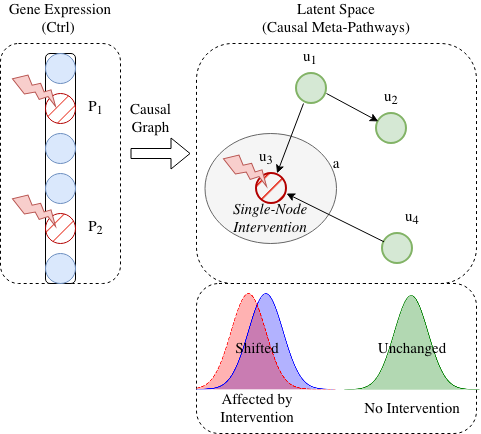
\includegraphics[width=0.98\linewidth]{gfx/Latent_interventions_modified.png}
    \caption{An intervention in gene expression $\variables$ shifts the conditional distribution $p^I(\latentcausalvar_i \mid \parentnodes(\latentcausalvar_i))$ of a single meta-pathway $\latentcausalvar_i$ (causal latent factor), while leaving unrelated latent factors unaffected.}\label{fig:single_node_intervention}
    \vspace{-\baselineskip}
\end{wrapfigure}
%
The central challenge of \gls{crl} is \emph{identifiability}: learning an encoder function $\practicalencoder$ that can uniquely recover the true causal latents $\latentcausalvars$ from the observations $\variables$.
However, when solely using observational data, this goal is theoretically intractable as multiple distinct causal structures
can generate identical observational distributions $\pdf{\variables}$~\citep{pearl2009causality, khemakhem2020variational}.
%
%Additionally, when using \gls{vae}s as the underlying architecture, \citet{khemakhem2020variational} showed that different parameter configurations can generate equivalent marginal distributions $\pdf{\variables}$, leaving the \gls{vae}-learned latent representations non-unique.
%
%In the causal setting, this problem is compounded, as multiple distinct causal structures can generate identical observational distributions.
%This means that learning interpretable causal mechanisms from observational data alone is ill-posed.
%
To overcome this, modern \gls{crl} relies on interventional data, as interventions create unique statistical signatures that break the symmetries present in observational data (Fig. \ref{fig:single_node_intervention}). Thus, identifiability depends on a set of key requirements (\citet{scholkopf2021toward}):

\textbf{Requirement 1 (Acyclic Causal Structure).}
The causal structure is assumed to form a \gls{dag}, a foundational principle in causal discovery~\citep{pearl2009causality}.

\textbf{Requirement 2 (Atomic Interventions).}
%Identifiability theory demonstrates that 
Causal structure recovery % (i.e., identifiability guarantee)
requires access to interventional data that targets each individual latent variable at least once. Atomic interventions are a key assumption in modern \gls{crl}~\citep{zhang2023identifiability, von2023nonparametric, de2025interpretable}.

% \begin{figure}[h]
%     \centering
%     \begin{minipage}{0.52\textwidth}
%         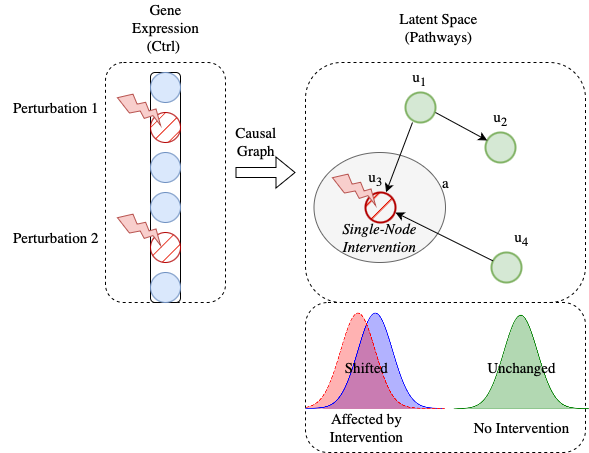
\includegraphics[width=\linewidth]{gfx/Latent_interventions.png}
%     \end{minipage}
%     \hfill
%     \begin{minipage}{0.40\textwidth}
%         \small
%         An intervention in the observed gene expression space $\variables$ causes a shift in a single latent pathway activity $\latentcausalvar_i$.
%         This alters the conditional distribution $p^I(\latentcausalvar_i \mid \parentnodes(\latentcausalvar_i))$ while leaving unrelated latent variables unaffected, a key requirement for identifiability.
%     \end{minipage}
%     \caption{Illustration of an atomic intervention in the latent space.}
%     \label{fig:single_node_intervention}
% \end{figure}

\textbf{Requirement 3 (Faithfulness).}
\gls{crl} also relies on the \emph{faithfulness assumption}, which posits that all conditional independencies in the data are a consequence of the causal graph structure (d-separation) and not due to coincidental cancellations of parameters \cite{zhang2023identifiability} %formalizes two key aspects of this requirement for their setting.
%First, \emph{linear interventional faithfulness} ensures that the effect of an intervention on a descendant is not perfectly cancelled by a linear combination of other variables.
%Second, they assume no perfect cancellation between a direct causal effect and other parallel paths in the graph.

Under these requirements, it is possible to provably recover the true latent causal graph up to a well-defined equivalence class.
Following the work of \citet{zhang2023identifiability}, their main theorem provides a formal guarantee for identifiability:

\begin{theorem}[Full DAG Identifiability, \citet{zhang2023identifiability}]
\label{thm:zhang_full_dag}
Assume a \gls{scm} with a latent \gls{dag} $\graph$ and an invertible mixing function.
If the set of interventions is atomic (targeting each latent variable at least once), and the assumptions of faithfulness hold, then the latent \gls{dag} $\graph$ and the intervention assignments are identifiable up to permutation, scaling, and translation (the CD-equivalence class).
\end{theorem}

The reliance on a \textbf{set of atomic interventions}, where each intervention targets a unique latent factor at least once, is the cornerstone of modern \gls{crl}-based prediction of genetic perturbations \citep{zhang2023identifiability,de2025interpretable}.

%-------------------------------------------------------------------------------
% Subsection: Soft Interventions in Biological Systems
%-------------------------------------------------------------------------------
% \subsection{Soft Interventions in Biological Systems}
% \label{subsec:background:soft_interventions}
% %-------------------------------------------------------------------------------

% An intervention is considered "hard" if it replaces the causal mechanism of a variable entirely (e.g., setting it to a constant), whereas a "soft" intervention only alters the functional relationship to its parent nodes.
% The latter case is particularly relevant for biological data from modern experimental techniques like Perturb-seq~\citep{norman2019exploring}.
% In these \emph{closed-world experiments}, the genetic target of each intervention is known \emph{a priori}, providing a clear causal anchor.

% The study by \citet{norman2019exploring} is a prime example of a soft, gain-of-function intervention.
% It employed a CRISPR activation (CRISPRa) system, which uses a deactivated Cas9 (dCas9) that cannot cut DNA.
% Instead, it recruits transcriptional activators to gene promoters, leading to graded, tunable increases in endogenous gene expression.
% Because this approach modulates gene function rather than ablating it completely, it aligns perfectly with the mathematical definition of a soft intervention.

%-------------------------------------------------------------------------------
% Subsection: The Intervention Spillover Problem
%-------------------------------------------------------------------------------
\subsection{Intervention spillover in dense encoders: challenges for identifiability}
\label{subsec:background:spillover}
%-------------------------------------------------------------------------------

While identifiability theory provides a strong theoretical foundation, a key challenge arises in recent \gls{crl} architectural choices: the \emph{intervention spillover problem}. This phenomenon occur when a single-variable intervention in the high-dimensional observation space $\variables$ is transformed into a multi-variable distributional shift in the lower-dimensional latent space $\latentcausalvars$, which is in  direct conflict with the atomic intervention requirement  (Requirement 2 in \cref{subsec:background:targeted_interventions}). This phenomenon is particularly concerning in genetic perturbation experiments, as interventions are applied to individual genes in the high-dimensional expression space, yet their effects propagate through the cell's regulatory network and manifest as coordinated changes across multiple biological processes. 

\textbf{It is thus crucial to ensure that, for each intervened gene, the sole (causal) latent factor associated with the intervention encompasses all relevant biological processes}. 
%For a more detailed theoretical analysis of this problem, see \cref{app:proofs:spillover}. 
%
%This issue stems from a d
% An \emph{Ideal Causal Encoder}, $\idealencoder$, would satisfy the atomic intervention requirement by ensuring that a single-gene intervention only alters the parameters for the distribution of a single causal latent variable $\causallatentchangeapprox = \idealencoder(\variables_{\text{int}}) - \idealencoder(\variables_{\text{obs}})$.
% Consequently, the expected change in the latent variables would be perfectly sparse, modelled, for example, as $\causallatentchangeideal = \maskvector \cdot \interventionstrength$, where $\maskvector$ is a one-hot vector identifying the single latent target and $\interventionstrength$ is the scalar strength of the intervention (see \cref{fig:single_node_intervention}).
As such, an \emph{Ideal Causal Encoder}, $\idealencoder$, must satisfy atomic intervention by ensuring that an intervention on a single gene generates a distributional effect on a sole latent factor, %yielding a perfectly sparse, manifesting a clean, single-variable intervention  
rather than a dense multi-variable distributional shift.
%
However, interventional encoders $\practicalencoder$ with dense architectures, like MLPs, possess a dense Jacobian matrix, which %meaning that % each component of the latent vector is a function of all input components.
%a sparse change in the input $\variables$ propagates through the network, and  
results in a dense output implicating multiple plausible latent targets. The model is thus forced to select a single ``best'' latent factor whose distribution to shift. This behavior has several critical implications for the reliability of the learned intervention targets (\cref{app:proofs:spillover} for the formal assumptions and the proof of incompatibility of dense architectures). Our proposed architecture, on the other hand, satisfies identifiability while still modeling complex gene-gene relations, by enforcing the mapping to a unique causal latent via preconditioning and a learned DAG. 
%For a mathematical formulation of this ideal behavior, , %and  we refer the reader to %\cref{app:proofs:spillover:setup}, \cref{app:proofs:spillover:assumptions}, and \cref{app:proofs:spillover:lemma_proof}.


%This forces the model to select the  to shift, even when the dense encoder output implicates multiple plausible targets.This means that the model is forced to choose the `best' single (latent) target whose distribution to shift from a dense output that suggests multiple viable targets. 
% Thus the resulting approximated latent change---defined as $\latentchangeapprox = \practicalencoder(\variables_{\text{int}}) - \practicalencoder(\variables_{\text{obs}})$---becomes non-optimal.
%
% This creates a fundamental incompatibility.
% Formally, the model must learn an intervention effect that reconstructs this observed latent change, typically by implicitly minimizing a loss function:
% \begin{equation}
%     \mathcal{L} = || \latentchangeapprox - (\maskvector \cdot \interventionstrength) ||^2
%     \label{eq:spillover_loss}
% \end{equation}
%
 
%First, models that use a softmax function for latent target identification must force a ``winner-take-all'' decision on a dense signal, potentially misattributing the primary causal effect.
%Further, while the perturbed gene is known \emph{a priori}, its associated latent factor is not, making the task of reliably discovering it from an entangled signal intractable.
%This reframes the primary modeling objective: the model should be designed not to explore for a latent target, but to accurately learn the magnitude of the intervention's effect on the causal representation.
%We provide an in-depth discussion about this problem in \cref{app:proofs:spillover}.
%
%In a variational context, the encoder parameterizes the posterior distribution over a set of learned (exogenous) latent variables, from which we sample $\latentvars$. The learned causal graph (the \gls{scm}) then operates on $\latentvars$ to model the causal relationships between the \cmps{} $\latentcausalvars$ (see \cref{eq:scm_general}).
%
%\revised{\textbf{Spillover problem in genetic perturbation prediction}. 
%\textbf{Intervention spillover in current models for genetic perturbation prediction.} 
%

%
%thus crucial to distinguish this intervention spillover, an artifact of dense encoders, from true biological correlation. High correlations between genes do not violate the single-node intervention requirement.
%Rather, dense encoders fail by transforming a sparse perturbation into a dense entry point in the latent space.

%-------------------------------------------------------------------------------
% Subsection: The Role of Prior Knowledge in Causal Modeling
%-------------------------------------------------------------------------------
%\subsection{The Dilemma of Prior Knowledge in Causal Discovery}
%\label{subsec:background:spectrum}
%-------------------------------------------------------------------------------

%\textbf{The dilemma of prior knowledge in causal discovery.} 
